\anachapter{Thermochimie à usage dans les batteries}
\label{chp:thermochimie}

\objectif{
\faBattery[0] Concepts généraux de thermochimie
\begin{itemize}[label=\faAngleRight]
\item Travail chimique et travail électrique ;
\item Différentielle totale exacte des fonctions d'états, relations entre les variables d'états conjuguées et les dérivées partielles premières des fonctions d'état ;
\item Expression intégrale de l'enthalpie libre ;
\item Expression de l'enthalpie libre de réaction ;
\item Potentiel chimique d'un gaz parfait et extension à tous les constituants.
\end{itemize}

\faBattery[2] Relation chimique fictive
\begin{itemize}[label=\faAngleRight]
\item Savoir utiliser des grandeurs de formation ou molaires pour établir les grandeurs de réaction ;
\item \'{E}tablir la relation entre grandeurs de réaction et force électromotrice ; 
\item Savoir discuter de l'influence de la température sur la force électromotrice.
\end{itemize}

\faBattery[4] Transfert de phase
\begin{itemize}[label=\faAngleRight]
\item \'{E}tablir l'expression de la différentielle de l'enthalpie libre entre deux phases s'échangeant des particules ;
\item \'{E}tablir l'expression liant la force électromotrice au potentiel chimique d'un constituant entre deux phases.
\end{itemize}
}

Contrairement aux systèmes thermodynamiques étudiés en première année, une cellule électrochimique ou batterie est un système \blancbis{fermé} capable de \blancbis{convertir} l'énergie chimique en énergie électrique (ou l'inverse). 

De ce fait, \blancbis{décrire mathématiquement} l'évolution de ces systèmes nécessite d'être capable de \blancbis{modéliser ces deux formes d'énergie}.

%\section{De l'énergie à la force électromotrice}

\section{Description d'une transformation chimique : le potentiel chimique}
Une batterie est un système thermodynamique fermé, qui \blancbis{reçoit ou donne} de l'énergie sous forme de \blancbis{chaleur}\mySideNote{\`{A} priori, vous avez dû remarquer que votre téléphone chauffait lors d'un usage intensif ou d'une charge sur secteur.} ou sous \blancbis{forme électrique} à l'extérieur.

De plus, les matériaux constituant les batteries forment un ensemble chimique complexe avec \blancbis{plusieurs} constituants chimiques, présents dans de \blancbis{multiples phases}. Prendre en compte cette complexité chimique rendra la description thermodynamique plus ardue que l'étude des systèmes de première année\mySideNote{Tous les outils introduis dans ce chapitre resserviront dans la suite de la scolarité et sont des concepts utilisables dans de nombreux contextes.}.

%Dans la suite, plusieurs notions nouvelles de thermodynamique qui réapparaitront tout au long de vos études\mySideNote{Tous les outils introduit dans ce chapitre reserviront dans la suite de la scolarité et sont des concepts extrêmement important pour tout individu voulant décrire rigoureusement la chimie.} permettant de décrire ces systèmes.

\subsection{Modélisation du système thermodynamique}

Afin de développer les principales formules, écrivons une forme générique d'équation de réaction comme : 

\begin{equation}
\nu_1 A_1 + \nu_2 A_2 + \ldots + \nu_N A_N = 0
\end{equation}

avec $\nu_k < 0$ (resp. $\nu_k > 0$) pour un réactif (resp. un produit).

Pour simplifier, on va considérer initialement que ce système est \blancbis{fermé} et comporte donc \blancbis{$N$ constituants} chimiques\mySideNote{$(A_1, A_2, \ldots A_N)$} dans une \blancbis{unique phase}. Ce système est mis en contact avec l'atmosphère (thermostat/barostat).

La réaction chimique est considérée comme une transformation monobare et monotherme.

\subsection{Travail chimique et potentiel chimique}

Le premier principe de la thermodynamique nous dit que pour un \blancbis{système physique}\mySideNote{Détente ou compression d'un gaz, échauffement d'un liquide$\ldots$} (sans réaction chimique), la variation d'énergie interne est dû aux échanges thermiques et au travail des forces de pression. Or, si on considère une transformation \blancbis{réversible}, le premier principe peut s'écrire comme\mySideNote{Si une transformation est réversible, alors 
\begin{align*}
\delta Q &\stackrel{\text{rev}}{=} T dS \\
\delta W_P &\stackrel{\text{rev}}{=} -P dV
\end{align*}
} : 
\begin{equation}
dU = T dS - P dV
\label{eq:PIT_phys}
\end{equation}



Par analogie avec la mécanique, il est possible de construire une grandeur analogue à la pression permettant de décrire l'évolution chimique d'un système. Cette grandeur, symboliée par la lettre $\mu$, est appelée potentiel chimique.

\begin{figure}[H]
\begin{minipage}{0.55\textwidth}
\subfloat[\label{fig:Chp1-02a}]{
\includegraphics[width=3cm]{Fig02a}}\hfill\subfloat[\label{fig:Chp1-02b}]{
\includegraphics[width=3cm]{Fig02b}}
\end{minipage}\hfill\begin{minipage}{0.40\textwidth}
\caption{\ref{fig:Chp1-02a} Représentation schématique de l'évolution d'un système mécanique composé de deux compartiments, séparé par une surface mobile, de volume $V_A$ et $V_B$, rempli de gaz à la pression $P_A$ et $P_B$ ; \ref{fig:Chp1-02b} Représentation schématique de l'évolution d'une réaction chimique \ce{{\color{blue} A} -> {\color{red}B}}.}
\end{minipage}
\end{figure}

Comme schématisé à la Fig. \ref{fig:Chp1-02a} la pression est la grandeur \blancbis{intensive} permettant de mesurer toutes les forces exercées par les particules de gaz de chacun des compartiments sur la surface mobile entre les compartiments A et B. La différence de pression permet donc de décrire l'évolution des volumes. Le potentiel chimique, représenté pour un système chimique à la Fig. \ref{fig:Chp1-02b}, est constuit de manière analogue.

Comme avec le travail des forces de pression, les thermodynamiciens définissent le travail chimique associé à chacun des constituants $j$ comme : 
\begin{equation}
\delta W_{\chi, j} \stackrel{rev}{=} \mu_j dn_j
\end{equation}

où $\mu_j$ est le potentiel chimique du constituant $j$.

\definition{
Le potentiel chimique représente "l'énergie potentielle" d'une mole de constituant $j$ dans le mélange au cours de la réaction chimique. 

~

Par analyse dimentionelle du travail, le potentiel chimique a pour unité \si{\joule\per\mole}.}



Pour un système, soumis à une transformation \blancbis{chimique réversible}, le premier principe permet d'écrire l'identité thermodynamique ci-dessous, dans laquelle a été ajouté le terme chimique à l'Eq. \ref{eq:PIT_phys} : 

\begin{equation}
dU = TdS - PdV + \sum_j \mu_j d n_j
\end{equation}
%par le système thermodynamique lorsqu'une mole de constituant est emmenée du vide dans une solution (solide, liquide).

%Il inclut le gain énergétique issu des interactions intermoléculaires et le gain entropique (augmntation du désordre) résultant de l'addition d'un constituant dans une phase.

\subsection{Forme différentielle des fonctions d'état}




\definition{
Dans le cas d'une transformation \blancbis{réversible} d'un système constitué de $N$ constituant chimique dans une phase, les identités thermodynamiques suivantes peuvent être écrites : 

\begin{align}
dU &= TdS - PdV + \sum_{j=1}^N \mu_j d n_j \label{eq:dU} \\
dH &= TdS + V dP + \sum_{j=1}^N \mu_j d n_j \label{eq:dH} \\
dG &= -S dT + V dP + \sum_{j=1}^N \mu_j d n_j \label{eq:dG}
\end{align}
}

Les fonctions d'états sont des fonctions à plusieurs variables : 

\begin{minipage}{0.45\textwidth}
\begin{tabular}{cc}
\toprule
Fonction d'état & Variables d'état \\
\midrule
U & $(S, V, n_1, \ldots, n_N)$ \\
H & $(S, P, n_1, \ldots, n_N)$ \\
G & $(T, P, n_1, \ldots, n_N)$ \\
\bottomrule
\end{tabular}
\end{minipage} \hspace{1cm} \begin{minipage}{0.45\textwidth}
\captionof{table}{Association de quelques fonctions d'état à leurs variables d'état naturelles.}
\end{minipage}

De ce fait, pour l'enthalpie libre, par exemple, on sait que l'on peut aussi écrire la différentielle totale exacte comme : 

\begin{equation}
dG = \left ( \frac{\partial G}{\partial T} \right )_{P, n_1, \ldots n_N} dT + \left ( \frac{\partial G}{\partial P} \right )_{T, n_1, \ldots n_N} dP + \sum_j \left ( \frac{\partial G}{\partial n_j} \right )_{T,P, n_{k \neq j}} d n_j
\label{eq:def_dG_totexact}
\end{equation}

On peut alors identifier avec la définition mathématique de la différentielle de G, Eq. \ref{eq:def_dG_totexact}, et le résultat issu du premier principe, Eq. \ref{eq:dG}, les dérivées suivantes\mySideNote{On peut lire que l'entropie est la variation de l'enthalpie libre avec la température lorsque la pression et la composition d'un mélange sont constants.} : 

\begin{center}
\begin{tabular}{ccc}
$\left ( \frac{\partial G}{\partial T} \right )_{P, n_1, \ldots n_N} = - S$ & $\left ( \frac{\partial G}{\partial P} \right )_{T, n_1, \ldots n_N} = V$ & $\left ( \frac{\partial G}{\partial n_j} \right )_{T,P, n_{k \neq j}} = \mu_j$ \\
\end{tabular}
\end{center}

Bien entendu, tout cela peut se résumer sur un tableau\mySideNote{Il est inutile d'apprendre ces dérivées par coeur, mais il faut savoir les retrouver facilement.} : 

\definition{
Les dérivées premières des fonctions d'état sont associées aux grandeurs, dites \blancbis{conjuguées}, des variables d'état de chaque fonction d'état. En écrivant la différentielle totale exacte et les résultats du premier principe de la thermodynamique, \blancbis{$3 (N + 2)$} dérivées premières peuvent être écrites : 
\begin{center}
\begin{tabular}{ccc}
$\left ( \frac{\partial U}{\partial S} \right )_{V, n_1, \ldots n_N} = T$ & $\left ( \frac{\partial U}{\partial V} \right )_{S, n_1, \ldots n_N} = -P$ & $\left ( \frac{\partial U}{\partial n_j} \right )_{S,V, n_k \neq n_j} = \mu_j$ \\
$\left ( \frac{\partial H}{\partial S} \right )_{P, n_1, \ldots n_N} = T$ & $\left ( \frac{\partial H}{\partial P} \right )_{S, n_1, \ldots n_N} = V$ & $\left ( \frac{\partial H}{\partial n_j} \right )_{S,P, n_k \neq n_j} = \mu_j$ \\
$\left ( \frac{\partial G}{\partial T} \right )_{P, n_1, \ldots n_N} = - S$ & $\left ( \frac{\partial G}{\partial P} \right )_{T, n_1, \ldots n_N} = V$ & $\left ( \frac{\partial G}{\partial n_j} \right )_{T,P, n_{k \neq j}} = \mu_j$ \\
\end{tabular}
\end{center}} 

\subsection{Définition intégrale de l'enthalpie libre}

\definition{Dans un système chimique composé de $N$ constituants, l'enthalpie libre est une fonction extensive définit sous forme intégrale par : 

\begin{equation}
G(T, P, n_1, .... n_N) = \sum_{j=1}^N \mu_j n_j
\end{equation}}

Une façon de parvenir intuitivement à ce résultat, est de se souvenir que l'enthalpie libre est une fonction \textbf{extensive}, c'est-à-dire que si je prends un système chimique et que je multiplie sa taille par deux, l'enthalpie libre est multipliée par deux.

\begin{minipage}{0.55\textwidth}

\includegraphics[width=8cm]{Fig03}
\end{minipage}\hfill\begin{minipage}{0.40\textwidth}
\captionof{figure}{Multiplication par deux d'un système chimique composé de deux constituants chimiques.}
\end{minipage}

Si on prend un système chimique quelconque et qu'on l'agrandit $\lambda$ fois, on s'attend à ce que l'enthalpie augmente $\lambda$ fois, soit l'égalité : 
\begin{equation}
G(T, P, \lambda n_1, .... \lambda n_N) = \lambda G(T, P, n_1, .... n_N)
\end{equation}

Naturellement, on en déduit alors que :
\begin{equation}
G(T, P, n_1, .... n_N) = \sum_j \mu_j n_j
\end{equation}

\subsection{Relation entre grandeurs de réaction et potentiel chimique}

\definition{
L'enthalpie libre de réaction est liée aux potentiels chimiques par la relation : 
\begin{equation}
\Delta_r G = \sum_j \nu_j \mu_j 
\end{equation}
}

Pour démontrer cette relation, il faut se rappeler qu'il est possible de décrire l'évolution du système lors d'une réaction chimique grâce à une unique variable : l'avancement chimique $\xi$, au lieu de considérer individuellement la variation de composition de chacun des constituants. Pour cela, dressons un tableau d'avancement : 

\begin{tabular}{cccccccc}
\toprule
 & $\nu_1 \ce{A_1}$ & + &  $\nu_2 \ce{A_2}$ & + & $\ldots$ & + & $\nu_N \ce{A_N}$ = 0 \\
\midrule
$t = 0$ & $n_1(0)$ & & $n_2(0)$ & & $\ldots$ & & $n_N(0)$ \\
$t > 0$ & $n_1(0) + \nu_1 \xi (t)$ & & $n_2(0) + \nu_2 \xi (t)$ & & $\ldots$ & & $n_N(0) + \nu_N \xi (t)$ \\
\bottomrule
\end{tabular}

On voir immédiatement que la seule variable temporelle $\xi$, d'où
\begin{align}
n_j (t) = n_j (0) + \nu_j \xi (t) \implies dn_j = \nu_j d\xi \label{eq:dnj}
\end{align}

Or, on peut écrire la première identité thermodynamique Eq. \ref{eq:dG} en y intégrant l'équation Eq. \ref{eq:dnj} : 

\begin{equation}
dG = -S dT + V dP + \left( \sum_j \nu_j \mu_j \right) d \xi
\end{equation}

Vous savez que par définition, l'enthalpie de réaction représente la variation de l'enthalpie libre avec l'avancement, soit : 

\begin{equation}
\Delta_r G = \left( \frac{\partial G}{\partial \xi } \right)_{T, P} \implies \Delta_r G = \sum_j \nu_j \mu_j
\end{equation}

\section{Expression, propriétés et utilisation du potentiel chimique}

\subsection{Expression}

\definition{
Le potentiel chimique d'un constituant $i$ dans une phase donnée est décrit par la forme analytique : 

\begin{equation}
\mu_i (T, P, a_i) = \mu_i^\circ (T) + RT \ln a_i
\end{equation}

où $a_i$ l'activité du constituant et $\mu_i^\circ$ est le potentiel chimique dans son état standard.}

Le potentiel chimique a une forme fonctionnelle inspirée d'un gaz parfait. Considérons un gaz parfait (nécessairement constitué d'une phase) constitué de $N$ constituants à la pression P et la température T. Le potentiel chimique du constituant $i$ est donné par : 

\begin{equation}
\mu_j = \left ( \frac{\partial G}{\partial n_j} \right )_{T,P, n_i \neq n_j}
\end{equation}

Dans le cas d'un gaz parfait, on peut montrer que : 

\begin{align}
\mu_j (T, P, x_j) &= \mu_j^\circ (T) + RT \ln \frac{P_j}{P^\circ} \\
&= \mu_j^\circ (T) + RT \ln x_j + RT \ln \frac{P}{P^\circ}
\end{align}

avec $P_i$ la pression partielle du gaz $i$ et $x_i$ la fraction molaire.

\example{
On sait qu'un gaz est constitué de $N$ constituants tel que : 
\begin{align}
\frac{\partial \mu_i}{\partial P} &=  \frac{\partial}{\partial P} \frac{\partial G}{\partial n_i} \\
&= \frac{\partial}{\partial n_i} \frac{\partial G}{\partial P} \quad \text{(car G est une fonction d'état)}\\
&= \frac{\partial}{\partial n_i} V \\
&= V_{m, i}
\end{align}

Or si les constituants sont des gaz parfaits, on sait que : $P_i V_{m,i} = RT$, d'où : 

\begin{align}
\frac{\partial \mu_i}{\partial P} &= \frac{RT}{P_i} \\
\int_{\mu_i^\circ (T)}^{\mu_i (T, P_i)} d\mu_i &= \int_{P^\circ}^{P_i} \frac{RT}{P'_i} d P'_i \\
\mu_i (T, P_i) - \mu_i^\circ (T) &= RT \ln \frac{P_i}{P^\circ}
\end{align}}

\subsection{Résultats importants}

\subsubsection{Influence de la température}

\definition{
Le potentiel chimique est une fonction de la température, dont la variation avec celle-ci est donnée par l'opposé de l'entropie molaire du constituant $j$ :

\begin{align}
\left( \frac{\partial \mu_j }{\partial T} \right)_{P, n_1, \ldots , n_N}= -S_{m,j}
\end{align}
}

Une simple étude de la valeur de l'entropie molaire d'un constituant vous permet donc de savoir à quel point celle-ci va diminuer l'énergie potentielle d'un constituant chimique.


\subsubsection{Expression de l'enthalpie libre de réaction}

\definition{
L'enthalpie de réaction est liée au quotient réactionnel $Q_r$ par la relation : 

\begin{equation}
\Delta_r G = \Delta_r G^\circ + RT \ln Q_r
\end{equation}


où $\Delta_r G^\circ$ est l'enthalpie standard de réaction, $T$ la température et $Q_r$ le quotient réactionnel.
}

Cette relation admise en BUT1 est un résultat très utile qui est une conséquence directe de la forme analytique du potentiel chimique.

\example{
On sait que :

\begin{equation}
\Delta_r G = \sum_i \nu_i \mu_i 
\end{equation}

On a alors : 

\begin{align}
\Delta_r G &= \sum_i \nu_i (\mu_i^\circ + RT \ln a_i) \\
 &= \sum_i (\nu_i \mu_i^\circ + RT \nu_i \ln a_i) \\
 &= \sum_i \nu_i \mu_i^\circ + RT \sum_i \ln a_i^{\nu_i} \\
 &= \underbrace{\sum_i \nu_i \mu_i^\circ}_{\Delta_r G^\circ} + RT \ln \underbrace{\prod_i a_i^{\nu_i}}_{Q_r}
\end{align}
}


\subsection{Application aux batteries : le transfert de phase}
%Warning Fig.

Le potentiel chimique est une grandeur particulièrement utile dans l'étude des batteries. En effet, il permet le plus souvent de ramener un problème complexe constitué de $N$ constituants chimique à l'étude de $N$ problèmes simple à $1$ constituant. Ainsi, à l'aide de cette grandeur, les chimistes des matériaux s'affranchissent de toute difficulté dans l'étude de leurs systèmes.

Dans une batterie, lors d'une décharge, on sait que deux phénomènes ont lieu simultanément : 
\begin{enumerate}
\item les électrons migrent du pôle $\ominus$ (anode) au pôle $\oplus$ (cathode) par les fils électriques ;
\item les cations migrent du pôle $\ominus$ au pôle $\oplus$ par l'électrolyte.
\end{enumerate}

Les chimistes des matériaux ramènent souvent l'étude complexe d'une réaction d'oxydoréduction au transport d'une espèce chimique.

\subsubsection{\'{E}tude de l'équilibre chimique}

On va formaliser les deux problèmes physiques ci-dessus de manière unique : une espèce \emph{A} migre de l'électrode $\oplus$ vers l'électrode $\ominus$ en passant par un milieu matériel, noté $m$.

\begin{minipage}{0.45\textwidth}

\includegraphics[width=6cm]{Fig04}
\end{minipage}\hfill\begin{minipage}{0.45\textwidth}
\captionof{figure}{Modélisation d'un transfert d'électron ou d'un transfert d'ion.}
\label{fig:Chp1-04}
\begin{equation*}
\ce{A(\oplus) <=> A(m) <=> A(\ominus)}
\end{equation*}
\end{minipage}

On sait que lors de l'étude d'un tel transfert, le système est composé de $N$ constituants répartis, cette fois-ci, \blancbis{plusieurs} phases. L'ensemble forme un système \emph{fermé}, mais il peut y avoir un \blancbis{transfert de matière} entre les différentes phases, comme illustré dans la Fig. \ref{fig:Chp1-04}.

Si on considère un transfert d'un constituant A entre les deux électrodes, le milieu matériel n'étant qu'un médiateur permettant ce transport, l'enthalpie libre, se réécrit alors comme : 
\begin{equation}
dG = -S dT + V dP + \sum_j \mu_j^\oplus dn_j^\oplus + \sum_j \mu_j^\ominus dn_j^\ominus
\end{equation}

En général, il va de soi que le milieu matériel ne constitue pas un "réservoir"\mySideNote{Un fil électrique ne permet pas de stocker des électrons par exemple} permettant de stocker les espèces qui migrent. On a alors nécessairement une équation de conservation de la matière : 
\begin{equation}
n_j^{tot} = n_j^\oplus + n_j^\ominus + n_j^m \implies dn_j^\oplus + dn_j^\ominus = 0
\end{equation}

qui permet de réduire l'enthalpie libre à : 
\begin{equation}
dG = -S dT + V dP + \sum_j (\mu_j^\oplus - \mu_j^\ominus) dn_j^\oplus
\end{equation}

\definition{On considère une transformation thermostatée et barostatée où une espèce \ce{A} migre du pôle $\oplus$ vers $\ominus$ suivant l'équation de réaction : 
\begin{align*}
\ce{A ( \oplus) <=> A (\ominus) }
\end{align*}

La variation d'enthalpie libre peut s'écrire : 


\begin{equation}
dG = \sum_j (\mu_j^\oplus - \mu_j^\ominus) dn_j^\oplus
\label{eq:dG_phasetransfert}
\end{equation}
}


\subsubsection{Conséquence}

Le second principe de la thermodynamique nous dit que pour une transformation monobare/monotherme (en l'absence de travail électrique), l'enthalpie libre décroit, soit que $dG < 0$. La relation Eq. \ref{eq:dG_phasetransfert} nous montre que : 
\begin{itemize}
\item $\mu_j^\oplus > \mu_j^\ominus$ le constituant $j$ est soumis à une "force chimique" qui le pousse à aller de l'électrode $\oplus$ à l'électrode $\ominus$ ; 
\item $\mu_j^\oplus < \mu_j^\ominus$ le constituant $j$ est soumis à une "force chimique" qui le pousse à aller de l'électrode $\ominus$ à l'électrode $\oplus$ ; 
\item $\mu_j^\oplus = \mu_j^\ominus$ le constituant $j$ est soumis à aucune force chimique.
\end{itemize}

Par force chimique qui le pousse à aller de l'électrode $\oplus$ à l'électrode $\ominus$, il est sous-entendu que le constituant $j$ est plus stable chimiquement dans la phase $\ominus$ et $\oplus$. Cette affinité chimique pour une phase plutôt que l'autre peut-être vu comme une force thermodynamique\mySideNote{Par analogie avec la force en mécanique.}.


\section{Travail électrique}

Tout le travail de construction du potentiel chimique nous a permis de montrer que le potentiel chimique constitue une mesure de la stabilité d'un constituant $j$ dans sa phase. Bien entendu, les espèces considérées dans une pile seront souvent \blancbis{chargées} et le travail électrique devra donc aussi être considéré dans le second principe.


\subsection{Définition}
Nous avons vu au chapitre précédent que le travail électrique, notée $W'$, s'écrit mathématiquement comme : 
\begin{equation}
W' = \int e dq
\end{equation}

où $e$ est la f.e.m. et $dq$ la variation de charge du système.

Afin de décrire ce système, on va considérer une forme plus habituelle de l'équation de réaction au sein de la cellule : 
\begin{align*}
\nu_1 A_1^{z_1} + \nu_2 A_2^{z_2} + \ldots + \nu_N A_N^{z_N} = 0
\end{align*}

où $(z_1, z_2 \ldots z_N)$ sont les charges formelles associées à chacune des entités rédox. De plus, on va considérer que $m e^-$ sont échangés entre les deux pôles de la cellule. 

\attention{Il est important de noter dès à présent que l'électron est une entité qui sera considérée à part par rapport aux autres constituants chimiques à présent. L'Eq. \ref{eq:dG_phasetransfert} sera réécrite : 
\begin{align*}
dG = \sum_j (\mu_j^\oplus - \mu_j^\ominus) \cdot dn^\oplus_j + ( \mu_e^\oplus - \mu_e^\ominus ) \cdot dn_e^\oplus
\label{eq:dG_phasetransfert_2}
\end{align*}}


\subsection{Relation à l'enthalpie libre}
Dans le cas d'une transformation chimique soumis à un travail électrique, le second principe de la thermodynamique permet d'écrire : 

\begin{equation}
dG = \delta W' = e dq
\end{equation}

Or si on s'intéresse à la variation de charge $dq$ au pôle $\oplus$, on peut écrire par exemple que : 
\begin{equation*}
dq = \sum_i (-z_i F) \cdot dn^\oplus_i - F \cdot dn^\oplus_e
\end{equation*}

On a alors une égalité intéressante entre le terme chimique et le terme électrique lorsque l'on est à l'équilibre chimique :
\begin{equation}
\sum_j (\mu_j^\oplus - \mu_j^\ominus) \cdot dn^\oplus_j + ( \mu_e^\oplus - \mu_e^\ominus ) \cdot dn_e^\oplus = \sum_i (- z_i F e) \cdot  dn^\oplus_i - F e \cdot dn^\oplus_e
\end{equation}

\definition{
On considère une transformation monobare et monotherme d'un système chimique composé de $N$ constituants où un échange de $m$ électrons a lieu entre deux électrodes. \`{A} l'équilibre chimique, on peut écrire pour chacun des constituants chimiques l'égalité suivante :

\begin{align*}
\mu_j^\oplus - \mu_j^\ominus = - z_j F e
\end{align*}

et écrire pour les électrons que : 

\begin{align*}
\mu_e^\oplus - \mu_e^\ominus = - F e
\end{align*}
}

L'un des points essentiels à noter dès à présent que la f.e.m. est une grandeur \blancbis{centrale} dans la description des cellules électrochimiques : sa simple valeur nous indique la stabilité de n'importe quel constituant chimique dans les différentes phases d'une cellule électrochimique. Or, la f.e.m. est liée à la réaction "fictive" de la cellule.


\begin{comment}
Or, en général, on cherche à décrire l'évolution de la charge avec la même variable que la partie chimique : l'avancement $\xi$.
\begin{equation}
dG = - z F e d\xi 
\end{equation}

\begin{boxedminipage}[t]{15cm}
On écrit la demi-équation rédox : 
\begin{equation}
\ce{Ox_1 = Red_1^{z+} + z e^-}
\end{equation}

On peut alors dresser un tableau d'avancement à partir de l'anode :
\begin{center}
\begin{tabular}{cccccccc}
\toprule
$t$ & \ce{Ox_1} & \ce{ = } & \ce{Red_1^{z+}} & + & \ce{z e^-} & Charges émis & Charges reçues \\
\midrule
$t=0$ & $n_0$ & & 0 & & 0 & 0 & 0\\
$t=\infty$ & $n_0 - \xi$ & & $n_0 + \xi$ & & $z \xi$ & $z F \xi$ & $-z F \xi$ \\
\bottomrule
\end{tabular}
\end{center}

On peut alors montrer que la variation de la quantité de charge reçue est donnée par : 
\begin{equation}
dq = F \cdot (-z d \xi) = -z F d\xi
\end{equation}

On a alors à partir du travail électrique, une nouvelle expression donnée par : 

\begin{equation}
dG = -z F e d\xi
\end{equation}
\end{boxedminipage}

\definition{Dans un système à pression et température constante, il est possible de lier l'enthalpie de réaction définie à l'Eq. \ref{} à la force électromotrice du système : 

\begin{equation}
\Delta_r G = -z F e
\end{equation}}

Dans ce genre de relation, on pose pour un système reversible, une juste proportionnalité entre la tension électrique du système et la variation d'énergie chimique au sein de deux demi-piles.
\end{comment}

\section{Réaction fictive d'une cellule électrochimique et force électromotrice}

\subsection{Relation entre l'enthalpie de réaction et la f.e.m.}

\definition{Dans une cellule électrochimique, dans laquelle on peut écrire une équation de réaction "fictive" de la forme :
\begin{equation}
\ce{\nu_1 A_1^{z_1} + \nu_2 A_2^{z_2} + \dots \nu_N A_N^{z_N} = 0}
\end{equation}

Dans une telle réaction, la variation d'enthalpie libre avec l'avancement est donnée par l'enthalpie libre de réaction $\Delta_r G$. Si on considère une transformation monobare et monotherme, la f.e.m. de la réaction est liée directement à l'enthalpie de réaction par la relation :

\begin{equation}
\Delta_r G = -m F e
\label{eq:DrG_fem}
\end{equation}

où $m$ est le nombre d'électrons échangé entre les pôles de la cellule.
}

On sait que l'enthalpie libre associée à un système thermostaté et barostaté, où un transformation chimique a lieu, peut s'écrire à l'aide des variables d'état $(T, P, \xi)$. 

L'enthalpie libre d'une telle réaction s'écrit : 
\begin{align*}
dG = -S dT + V dP + \Delta_r G d \xi
\end{align*}

De ce fait, si cette réaction reçoit un travail électrique $\delta W'$, on peut alors utiliser le second principe de la thermodynamique : 

\begin{align*}
dG \stackrel{\text{rev}}{=} -m F e d\xi
\end{align*}

\`{A} (T, P) constant, on en déduit alors l'Eq. \ref{eq:DrG_fem}.


\subsection{Relation entre f.e.m. et grandeurs de référence}

La relation \ref{eq:DrG_fem} est très utile car elle permet d'établir une relation simple entre l'enthalpie libre de la réaction "fictive" de la cellule électrochimique et la f.e.m. de la cellule.

En $BUT1$, les lois de Hess ont été établies afin de lier la détermination des grandeurs standard de n'importe quelle réaction aux réactions de formation des constituants de la réaction.

\subsubsection{Utilisation de la loi de Hess}

La loi de Hess permet de remonter aux grandeurs de réaction à partir de valeurs tabulées : l'enthalpie de formation standard $\Delta_f H^\circ$ et l'entropie molaire standard $S_m^\circ$.

\begin{align}
\Delta_r H^\circ &= \sum_j \nu_j \Delta_f H_j^\circ \\
\Delta_r S^\circ &= \sum_j \nu_j S_{m,j}^\circ \\
\Delta_r G^\circ &= \sum_j \nu_j \Delta_f G_j^\circ
\end{align}

Ces lois de Hess permettent de remonter à la force électromotrice $e^\circ$ dans des conditions standard : 

\begin{equation}
e^\circ (T) = - \frac{\Delta_r G^\circ}{mF}
\end{equation}

\exercice{
Dans le domaine médical, la pile $\ominus ~ \ce{Li} | \text{electrolyte} | \ce{I_2} ~ \oplus$ est utilisée comme source d'énergie pour les pacemakers. 

\Q Donner les demi-équations rédox associées à l'anode et la cathode, et en déduire l'équation de réaction.
\Q Calculer l'enthalpie standard de réaction à \SI{298}{\kelvin}.
\Q Calculer l'entropie standard de réaction à \SI{298}{\kelvin}.
\Q En déduire l'enthalpie libre de réaction à \SI{298}{\kelvin} puis déterminer la f.e.m dans ces conditions.

Dans ce dispositif, la tension de sortie a été mesurée en fonction de la quantité de charge déchargée. 

\begin{minipage}{0.55\textwidth} 

\includegraphics[width=\textwidth]{Fig06}
\end{minipage} \hfill \begin{minipage}{0.40\textwidth} 
\captionof{figure}{\'{E}volution de la tension de sortie et de la résistance interne d'une batterie \ce{Li}/\ce{I2} utilisée dans les pacemakers.}
\label{fig:Chp1-06}
\end{minipage}

\Q Montrer l'accord entre vos grandeurs et la mesure sur la majorité du cycle de décharge de la pile. 
\Q En vous appuyant sur l'équation de réaction, lier l'écroulement du potentiel de réaction au-delà de \SI{1.2}{\ampere\hour} à la structure de la pile.

~

\textbf{Données}
\begin{center}
\begin{tabular}{ccccc}
 & & Li & \ce{I2} & \ce{LiI} \\
Enthalpie de formation & [\si{\kilo\joule\per\mole}] & 0 & 0 & -270.1\\
Entropie molaire & [\si{\joule\per\mole\per\kelvin}] & 29.08 & 116.14 & 85.77 \\
\end{tabular}
%Table 2.1, advanced battery.
\end{center}}


\subsubsection{\'{E}tude de l'influence de la température}

Dans les cellules électrochimiques, l'étude de l'influence de la température est extrêmement importante pour comprendre la tenue thermique d'une cellule. Les lois de Hess permettent de remonter à la force électromotrice $e^\circ$ dans des conditions standard : 

\begin{equation}
e^\circ (T) = \frac{\Delta_r S^\circ}{mF} T - \frac{\Delta_r H^\circ}{mF}
\end{equation}

Pour une variation modérée de température, on peut souvent se placer dans l'approximation d'Ellingham, ce qui permet d'écrire que : 

\begin{equation}
\frac{d e^\circ}{dT} = \frac{\Delta_r S^\circ}{mF}
\end{equation}

Cette grandeur est appelée c{\oe}fficient thermique de la cellule.

\exercice{
On se placera dans l'approximation d'Ellingham.
\Q En déduire la relation entre la variation de la force électromotrice $e^\circ$ avec la température.
\Q Commenter et justifier la valeur obtenue.}

\subsection{D'où vient la relation de Nernst ?}

En supposant un système réversible, composé d'une pile fictive suivante : 

\begin{equation}
\ominus \quad \ce{Pt (s)} | \ce{Ox_1 (\phi)}; \ce{Red_1 (\phi)} || \ce{H^\oplus (aq)} | \ce{H2 (g)} | \ce{Pt (s)} \quad \oplus
\label{eq:pileOxRedvsESH}
\end{equation}
où $\phi$ indique la phase et \ce{Ox_1}/\ce{Red_1} indique un couple oxydant/réducteur quelconque. L'équation de réaction de cette pile est donnée par : 

\begin{center}
\begin{minipage}{0.4\textwidth}
\begin{align*}
\ce{Red_1 (\phi) &= Ox_1 (\phi) + m e^-} \\
\ce{H^+ (aq) + e^- &= H_2 (aq)} \quad \times m \\
\hline
\ce{m H^+ (aq) + Red_1 (\phi) &= \frac{m}{2} H_2 (g) + Ox_1 (\phi)}
\end{align*}
\end{minipage}
\end{center}

Dans ce système, la cathode est une électrode standard à hydrogène (ESH)

\begin{align}
\underbrace{\Delta_r G}_{-m F e} & = \underbrace{\Delta_r G^\circ}_{-m F e^\circ} + RT \ln Q_r \\
e &= e^\circ - \frac{RT}{mF} \ln Q_r \\
\end{align}

Or on sait que la force électromotrice est donnée par : 
\begin{align}
e &= E_\oplus - E_\ominus \\
&= E ( \ce{H^+} / \ce{H2} ) - E ( \ce{Ox_1} / \ce{Red_1} )
\end{align}

Or, on sait que l'ESH, référence absolue des potentiels, est définie par les hypothèses suivantes :
\begin{itemize}
\item $E^\circ ( \ce{H^+} / \ce{H2} ) = 0 $ (convention de Latimer) ;
\item l'activité du proton vaut 1 : $a (\ce{H^+}) = 1$ ;
\item l'activité du dihydrogène vaut 1 $a (\ce{H2}) = 1$.
\end{itemize}

Dans ces conditions, le potentiel cathodique vaut $E_\oplus = E ( \ce{H^+} / \ce{H2} ) = 0 $ ce qui sert de référence à tous les potentiels d'électrodes. Dans ce système, on retrouve alors l'équation de Nernst qui permet de retrouver le potentiel d'électrode par rapport au couple \ce{H^+}/\ce{H2}.

\definition{
Le potentiel d'électrode est donné par l'équation de Nernst définie comme : 
\begin{equation}
E ( \ce{Ox_1} / \ce{Red_1} ) = E^\circ ( \ce{Ox_1} / \ce{Red_1} ) + \frac{RT}{mF} \ln \frac{a^{|\nu_{Ox}|}(\ce{Ox_1})}{a^{|\nu_{Red}|}(\ce{Red_1})}
\end{equation}
où $m$ indique le nombre d'électrons échangés.}

\newpage

\definition{
\begin{center}
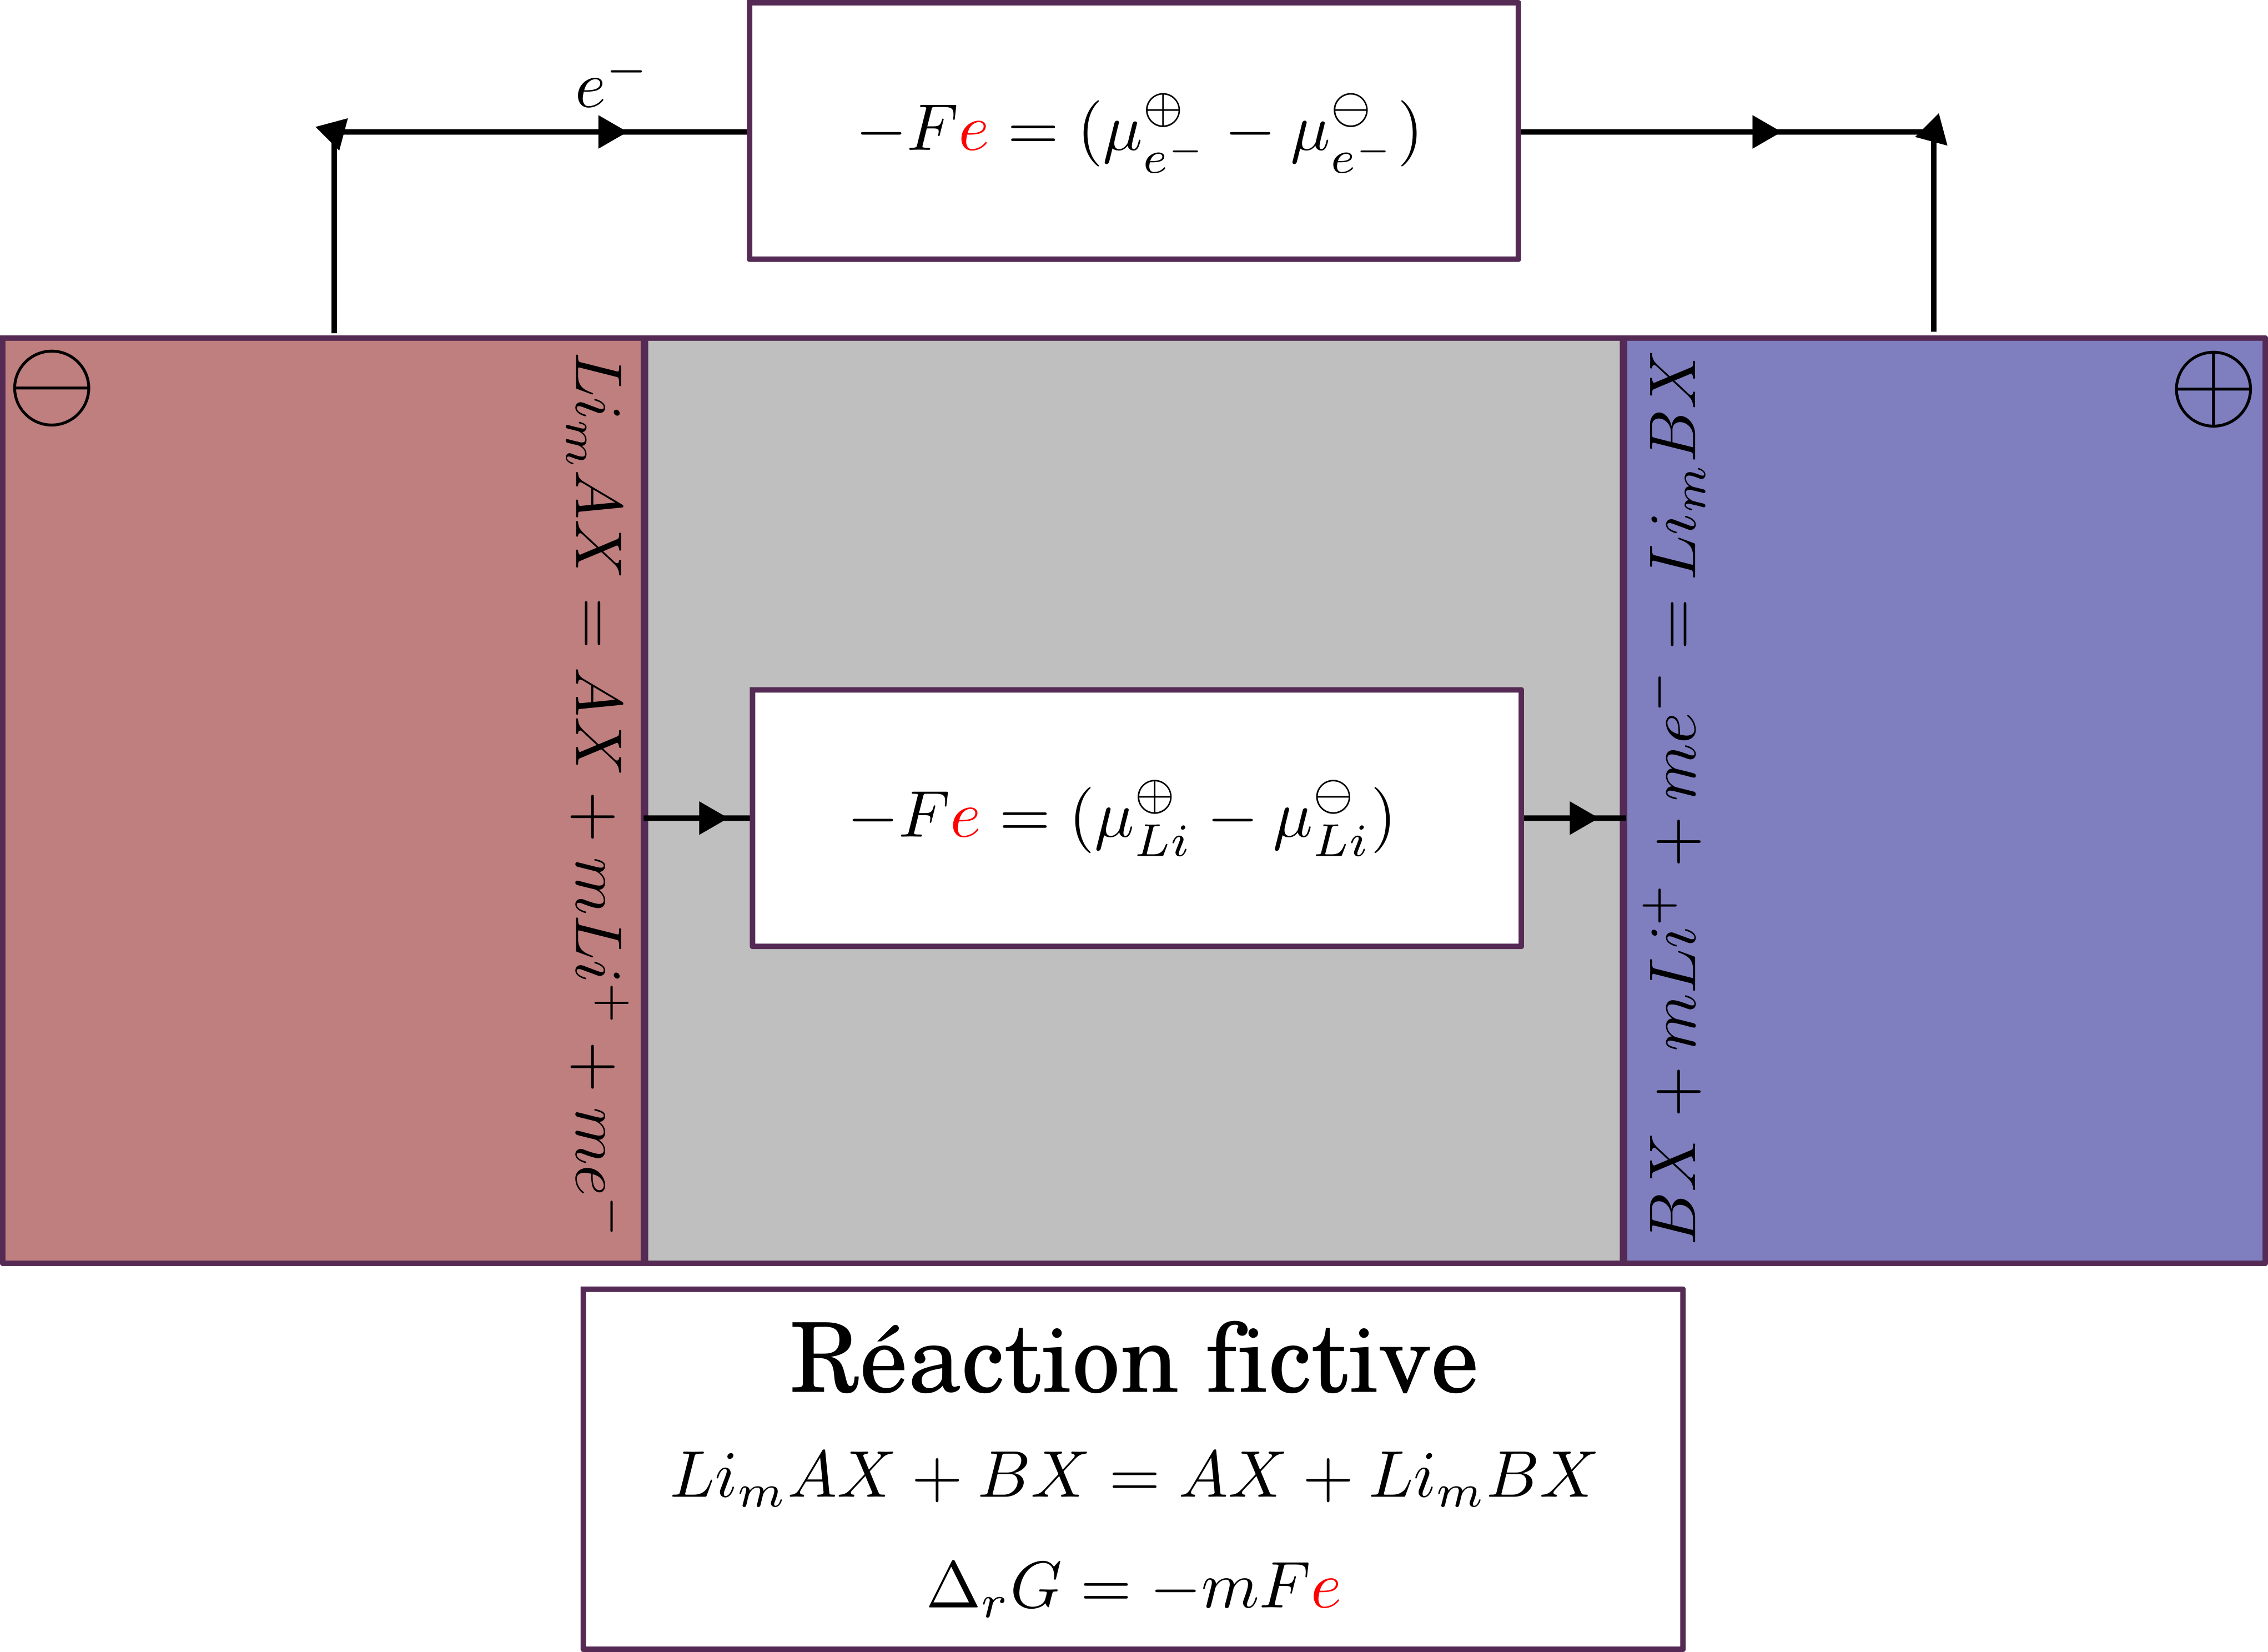
\includegraphics[width=0.8\textwidth]{figures-Chp1/Fig07}
\captionof{figure}{Résumé des relations clefs, utilisés dans le domaine des batteries, lors de la décharge d'un accumulateur au lithium composé de deux matériaux d'insertion aux pôles.}
\end{center}
Dans ce chapitre, on est parvenu à montrer que la force électromotrice est la grandeur thermodynamique qui permet de relier trois phénomènes : 
\begin{itemize}
\item la réaction fictive ;
\item le "transfert de phase" de l'électron ;
\item le "transfert de phase" du lithium.
\end{itemize}
Ces différentes relations, comme nous le verrons aux chapitres suivants, sont autant de points de vue possibles pour un chimiste d'interpréter les phénomènes chimiques à l'origine des variations de la f.e.m. 
}

%https://www.youtube.com/watch?v=7Wds1UdtOqc&ab_channel=PhysicalChemistry
\begin{comment}
\exercice{Donner la variance de quelques systèmes solides :
\begin{itemize}
\item donner la variance d'un alliage de bronze (solution solide de Cu et Zn)

\begin{boxedminipage}[t]{15cm}
\begin{align*}
X =4 &: P, T, \mu_{Cu}, \mu_{Zn} \\
Y =3 &: \text{1 phase solide} \\
v &= 3
\end{align*}
Un bronze stable est décrit à l'équilibre par (P, T, $x_{Cu}$).
\end{boxedminipage}

\end{itemize}}



\begin{boxedminipage}[t]{15cm}
Prenons-le cas de la pile $\ominus ~ \ce{Li} | \text{electrolyte} | \ce{I_2} ~ \oplus$, on peut alors écrire les différentes phases : 

On peut alors interpréter l'enthalpie libre de réaction par : 
%\begin{equation}
%\Delta_r G^\circ = \mu (\ce{LiI}) - \mu(\ce{Li}) - \frac{1}{2} \mu ( \ce{\LiI} )
%\end{equation}

\end{boxedminipage}
\end{comment}


%https://www.youtube.com/watch?v=4-1psMHSpKs&ab_channel=TheLimitingFactor

%https://www.college-de-france.fr/fr/agenda/cours/electrochimie-appliquee-les-differents-systemes-de-batteries/la-technologie-ion-lithium-son-origine-son-evolution-ses-dernieres-avancees-et-son-futur

%https://www.youtube.com/watch?v=DBLHaLhyo2w&ab_channel=BillyWu
